\documentclass[11pt]{article}
\usepackage[textwidth=18.0cm, textheight=23.0cm, top=2.0cm]{geometry}
\usepackage{pst-all}
\usepackage{amssymb}
\usepackage{tikz}
\usepackage{underscore}\begin{document}
\pagestyle{empty}


ClassName: \underline{\textbf{Class_04.2bp-4}}
\par
BinSize: \underline{\textbf{100 × 100}}
\par
ReduceSize: \underline{\textbf{100 × 100}}
\par
TypeNum: \underline{\textbf{20}}
\par
Num: \underline{\textbf{20}}
\par
OutS: \underline{\textbf{10000}}
\par
InS: \underline{\textbf{5520}}
\par
Rate: \underline{\textbf{0.552}}
\par
UB: \underline{\textbf{1}}
\par
LB0: \underline{\textbf{1}}
\par
LB: \underline{\textbf{1}}
\par
LBWithCut: \underline{\textbf{1}}
\par
NodeCut: \underline{\textbf{0}}
\par
ExtendedNodeCnt: \underline{\textbf{1}}
\par
GenNodeCnt: \underline{\textbf{1}}
\par
PrimalNode: \underline{\textbf{0}}
\par
ColumnCount: \underline{\textbf{1}}
\par
TotalCutCount: \underline{\textbf{0}}
\par
RootCutCount: \underline{\textbf{0}}
\par
LPSolverCnt: \underline{\textbf{1}}
\par
PricingSolverCnt: \underline{\textbf{0}}
\par
BranchAndBoundNum: \underline{\textbf{1}}
\par
isOpt: \underline{\textbf{true}}
\par
TimeOnPrimal: \underline{\textbf{0.000 s}}
\par
TimeOnPricing: \underline{\textbf{0.000 s}}
\par
TimeOnRmp: \underline{\textbf{0.063 s}}
\par
TotalTime: \underline{\textbf{0.141 s}}
\par
\newpage


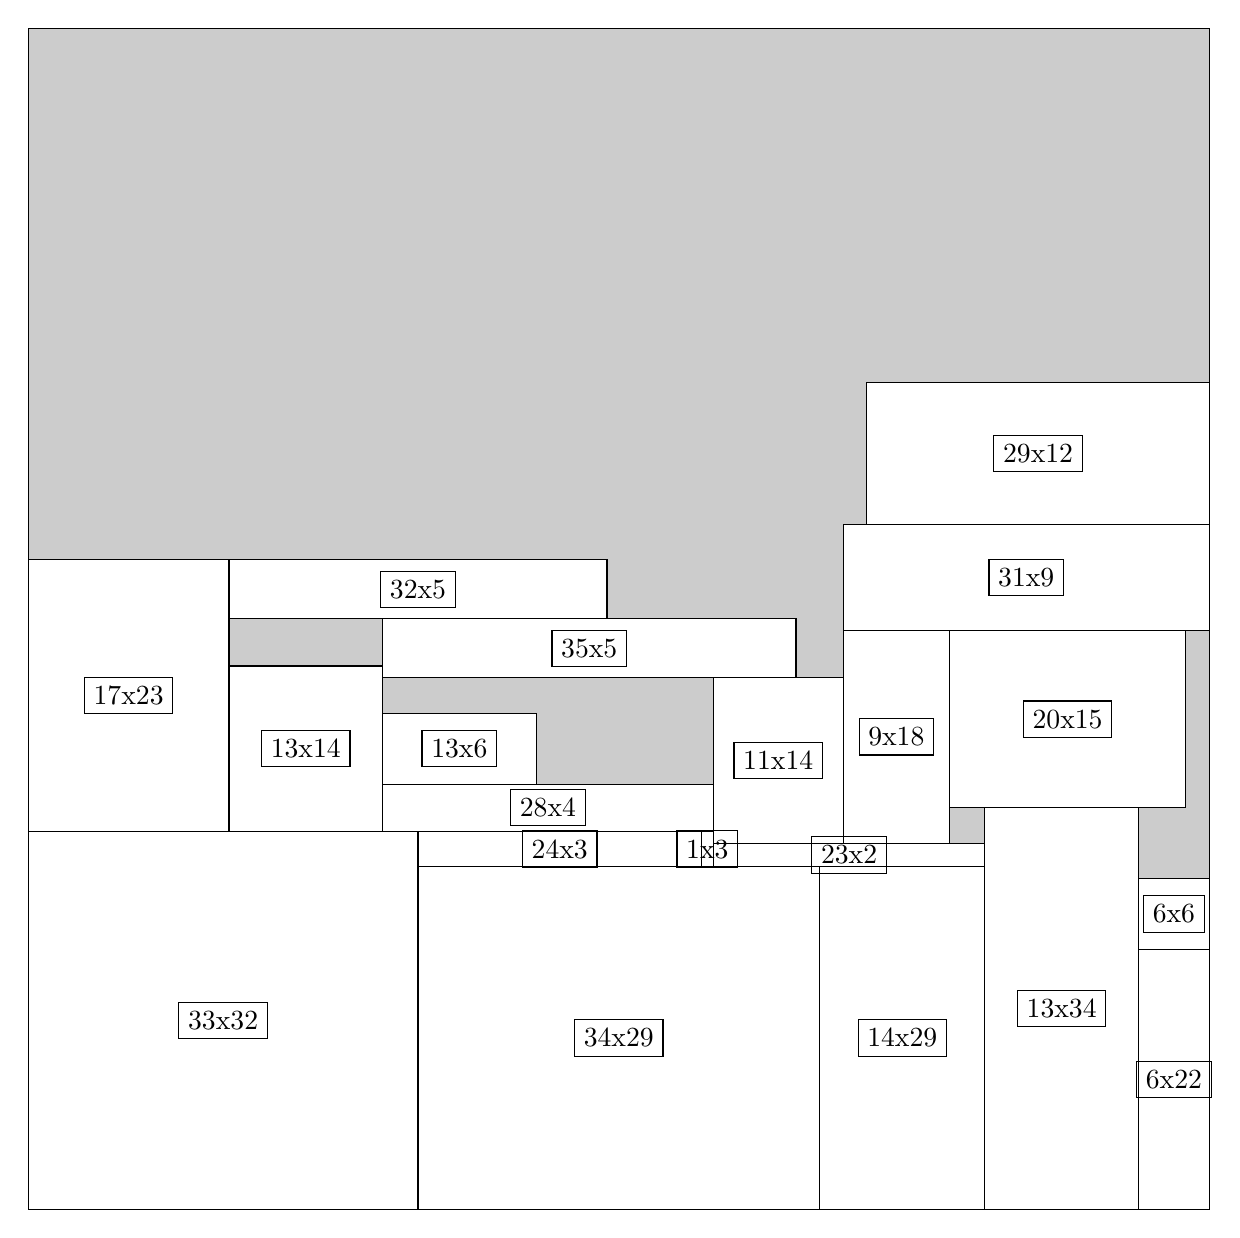
\begin{tikzpicture}[shorten >=1pt,scale=1.0,every node/.style={scale=1.0},->]
\tikzstyle{vertex}=[circle,fill=black!25,minimum size=14pt,inner sep=0pt]
\filldraw[fill=gray!40!white, draw=black] (0,0) rectangle (15.0,15.0);
\foreach \name/\x/\y/\w/\h in {33x32/0.0/0.0/4.95/4.8,34x29/4.95/0.0/5.1/4.35,13x34/12.15/0.0/1.95/5.1,11x14/8.7/4.6499999999999995/1.65/2.1,17x23/0.0/4.8/2.55/3.4499999999999997,29x12/10.65/8.7/4.35/1.7999999999999998,20x15/11.7/5.1/3.0/2.25,31x9/10.35/7.35/4.6499999999999995/1.3499999999999999,13x14/2.55/4.8/1.95/2.1,35x5/4.5/6.75/5.25/0.75,9x18/10.35/4.6499999999999995/1.3499999999999999/2.6999999999999997,32x5/2.55/7.5/4.8/0.75,14x29/10.049999999999999/0.0/2.1/4.35,6x22/14.1/0.0/0.8999999999999999/3.3,28x4/4.5/4.8/4.2/0.6,13x6/4.5/5.3999999999999995/1.95/0.8999999999999999,24x3/4.95/4.35/3.5999999999999996/0.44999999999999996,23x2/8.7/4.35/3.4499999999999997/0.3,6x6/14.1/3.3/0.8999999999999999/0.8999999999999999,1x3/8.549999999999999/4.35/0.15/0.44999999999999996}
\filldraw[fill=white!40!white, draw=black] (\x,\y) rectangle node[draw] (\name) {\name} ++(\w,\h);
\end{tikzpicture}


w =33 , h =32 , x =0 , y =0 , v =1056
\par
w =34 , h =29 , x =33 , y =0 , v =986
\par
w =13 , h =34 , x =81 , y =0 , v =442
\par
w =11 , h =14 , x =58 , y =31 , v =154
\par
w =17 , h =23 , x =0 , y =32 , v =391
\par
w =29 , h =12 , x =71 , y =58 , v =348
\par
w =20 , h =15 , x =78 , y =34 , v =300
\par
w =31 , h =9 , x =69 , y =49 , v =279
\par
w =13 , h =14 , x =17 , y =32 , v =182
\par
w =35 , h =5 , x =30 , y =45 , v =175
\par
w =9 , h =18 , x =69 , y =31 , v =162
\par
w =32 , h =5 , x =17 , y =50 , v =160
\par
w =14 , h =29 , x =67 , y =0 , v =406
\par
w =6 , h =22 , x =94 , y =0 , v =132
\par
w =28 , h =4 , x =30 , y =32 , v =112
\par
w =13 , h =6 , x =30 , y =36 , v =78
\par
w =24 , h =3 , x =33 , y =29 , v =72
\par
w =23 , h =2 , x =58 , y =29 , v =46
\par
w =6 , h =6 , x =94 , y =22 , v =36
\par
w =1 , h =3 , x =57 , y =29 , v =3
\par
\newpage


\end{document}